\section{Funções Vetoriais}

\subsection*{Definição de funções Vetoriais}
\begin{frame}[label=fun-vet]{Funções Vetoriais}
\begin{defin}
Uma \dt{função vetorial} é uma função cujo domínio é um conjunto de números reais e cuja imagem é um conjunto de vetores em $\R^n$, denotada por:
\[\begin{array}{lcl}
\vec{r}: & D\subset \R &  \longrightarrow \R^n\\
         & t           & \longmapsto \vec{r}(t)=(f_1(t),f_2(t),\ldots,f_n(t)).
\end{array}\]

As funções $f_1,\ldots,f_n$ são chamada \dt{funções componentes}.
\end{defin}

\begin{example}
\begin{enumerate}
\item $\vec{r}(t)=(t,t)$, $t\in \R$.
\item $\vec{r}(t)=(t,1,0)$, $t\geq 0$.
\end{enumerate}
\end{example}

\end{frame}


\subsection*{limite e continuidade}
\begin{frame}[label=fun-vet]{Limite e Continuidade}
\begin{defin}
Sejam $\vec{r}(t)=(f_1(t),f_2(t),\ldots,f_n(t))$ uma função vetorial com domínio $D$. Definimos o \dt{limite de $\vec{r}(t)$ quanto $t$ tende a $a\in D$} por 
\[\lim\limits_{t\to a}\vec{r}(t)=\left(\lim\limits_{t\to a}f_1(t),\ldots,\lim\limits_{t\to a}f_n(t)\right), \]
desde que o limite das funções componentes existam.
\end{defin}

\begin{exer}
Determine $\lim\limits_{t\to 0}\vec{r}(t)$, onde $\vec{r}(t)=(1+t^3, te^{-t})$.
\end{exer}


\end{frame}

\begin{frame}[label=fun-vet]
\begin{defin}
Uma função vetorial $\vec{r}$ é \dt{contínua em $a$} se $\lim\limits_{t\to a}\vec{r}(t)=\vec{r}(a)$.
\end{defin}
Em vista desta definição, uma função $\vec{r}$ é {\color{blue}contínua em $a$} se, e somente se, cada uma de suas {\color{blue}componentes é contínua em $a$}.



\end{frame}

\subsection*{Curvas Parametrizadas}
\begin{frame}[label=fun-vet]{Curvas Parametrizadas no plano}
Quando uma função vetorial \dt{$\vec{r}(t)=(f(t),g(t))$}, está definida em um intervalo $I$ da reta e  é \dt{contínua}, então o conjunto {\color{red}$C$} de todos os pontos $(x,y)$ do plano tais que
\begin{equation}\label{parametricas}
x=\dt{f(t)}\ \text{ e } y=\dt{g(t)}
\end{equation}
quando $t$ varia formam uma {\color{red}curva no plano}. As equações em  {\color{red} \eqref{parametricas}} são ditas {\color{red} equações paramétricas de $C$}, $\dt{\vec{r}}$ é dita ser uma {\color{red}parametrização de $C$} e $t$ é chamado de  {\color{red} Parâmetro}.
\begin{exe}
Determine as curvas parametrizadas por:
\begin{enumerate} 
\item $\vec{r}(t)=(\cos(t),\sin(t))$, $t\in [0,2\pi]$.
\item $\vec{r}(t)=(\cos(2t),\sin(2t))$, $t\in [0,2\pi]$.

\end{enumerate}
\end{exe}

Veja como plotar curvas parametrizadas usando python \href{https://reginaldodr.github.io/academic/posts/curvas-parametricas/curvas-parametricas.html}{\beamergotobutton{Link}}

\end{frame}

\begin{frame}[label=fun-vet]
\begin{block}{Parametrização de Função}
O gráfico de qualquer função $y=f(x)$ pode ser parametrizado de forma natural usando a variável $x$ como parâmetro, da seguinte forma:
\[\vec{r}(t)=(t,f(t)),\ t\in I.\]
\end{block}

\begin{exer}
 Determine uma parametrização para a parábola $y=x^2$.
\end{exer}
\end{frame}


\begin{frame}[label=fun-vet]
	\begin{casa}
		\begin{enumerate}
			\item  Determine uma parametrização para o segmento de reta que entre os pontos $(1,0)$ e $(2,5)$.
			\item Determine a curva parametrizada por $\vec{r}(t)=(2\cos(t),\sin(t))$, $t\in [0,2\pi]$.
		\end{enumerate}
	\end{casa}
\end{frame}

%---------------  coordenadas polares



\begin{frame}[label=fun-vet]{Coordenadas Polares}

		Um sistema de \dt{coordenadas polares} é estabelecido ao escolhermos um ponto no plano, conhecido como \dt{polo} (ou origem), denotado por $O$, e uma semi-reta começando em $O$, chamada \dt{eixo polar}. Qualquer ponto $P$ do plano é associado a um par ordenado $(r,\theta)$, chamado \dt{coordenadas polares} de $P$, sendo $r$ a distância de $P$ a $O$ e $\theta$ o ângulo entre o eixo polar e a reta $OP$.
		\medskip

\centering
\begin{tikzpicture}
\tikzset{>=latex}

\coordinate (A) at ({2*cos(45)},{2*sin(45)});
\coordinate (O) at (0,0);
\coordinate (i) at (2,0);

\pic[draw,angle eccentricity=1.5,->] {angle = i--O--A};

\draw[->] (0,0) -- (3,0) node[right] {eixo polar};

\node[thick] at (0.8,0.3) {$\theta$};
\draw[very thick,blue] (0,0) -- ({2*cos(45)},{2*sin(45)});

\node at (0.5,1) {$r$};
\node[right] at (A) {$(r,\theta)$};
\fill[red] (A) circle (2pt);

\node[left] at (0,0) {$O$};
  
\end{tikzpicture}


		\end{frame}
		

\begin{frame}[label=fun-vet]{Coordenadas Polares}
Usamos a convenção de que um ângulo é positivo se for medido no sentido anti-horário a partir do eixo polar e negativo se for medido no sentido horário. Se $P=O$, então $r=0$, e convencionamos que $(0,\theta)$ representa o polo para qualquer valor de $\theta$.
\medskip

No caso $r<0$, convencionamos que a coordenada $(r,\theta)$ corresponde ao simétrico, em relação à origem, do ponto $(|r|,\theta)$.

\centering

\begin{tikzpicture}
\tikzset{>=latex}

\coordinate (A) at ({2*cos(45)},{2*sin(45)});
\coordinate (O) at (0,0);
\coordinate (i) at (2,0);
\coordinate (B) at ({2*cos(45+180)},{2*sin(45+180)});

\pic[draw,->,angle radius=1cm] {angle = i--O--A};

\pic[draw,->] {angle = i--O--B};

\draw[->] (0,0) -- (3,0) node[right] {eixo polar};

\node[thick] at (1.2,0.3) {$\theta$};
\draw[very thick,dashed] (0,0) -- ({2*cos(45)},{2*sin(45)});

\node at (0.5,1) {$r$};
\node[right] at (A) {$(r,\theta)$};
\fill[black] (A) circle (2pt);

\node[below] at (0,0) {$O$};

\draw[very thick,blue] (0,0) -- ({2*cos(45+180)},{2*sin(45+180)});

\node[left] at (B) {$(-r,\theta)$};
\fill[red] (B) circle (2pt);
\node at ({0.8*cos(90+45)},{0.8*sin(90+45)}) {$\theta +\pi$};
  
\end{tikzpicture}



\end{frame}
		
		\begin{frame}[label=fun-vet]
				\begin{exe}
					Marque os pontos cujas coordenadas polares são dadas
					\begin{multicols}{4}
						\begin{enumerate}[a]
							\item $(1,5\pi/4)$
							
							\item $(2,3\pi)$
							
							\item  $(2,-2\pi/3)$
							
							\item $(-3,3\pi/4)$  \medskip
						\end{enumerate}
					\end{multicols}
				\end{exe}

\begin{center}
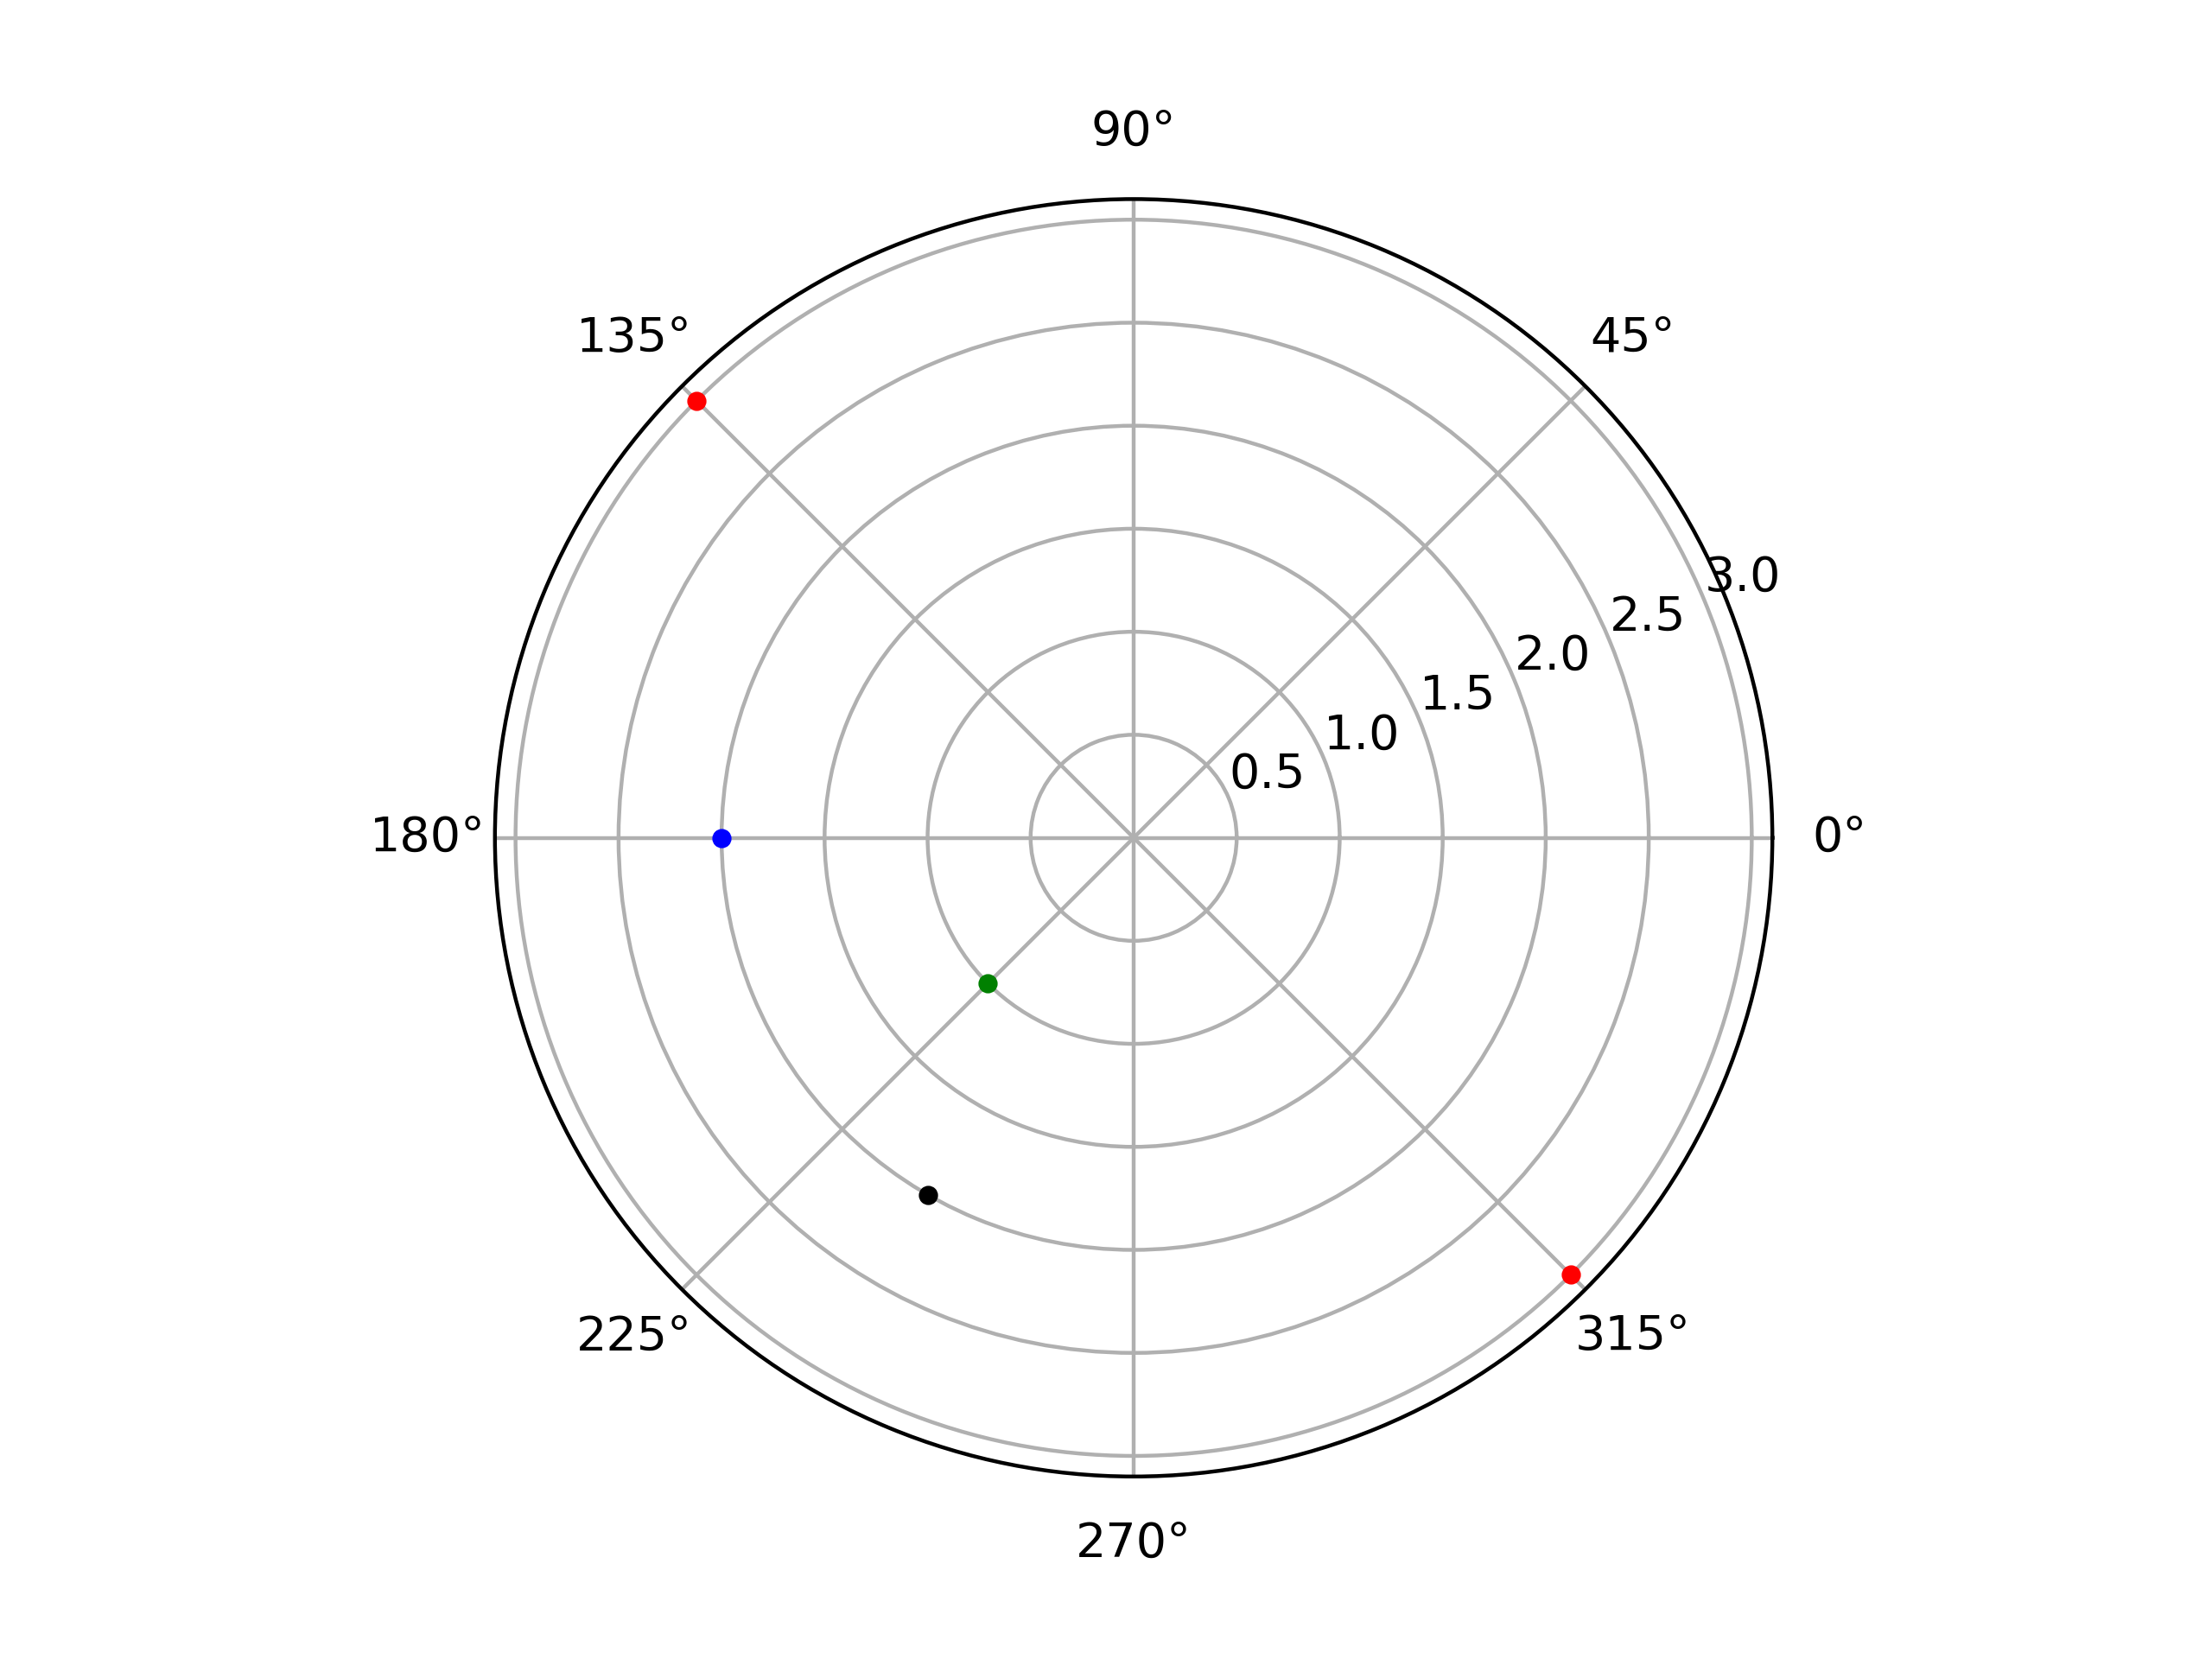
\includegraphics[scale=.5]{figuras/polar1.png}
\end{center}

		\end{frame}

\begin{frame}[label=fun-vet,fragile=singleslide]
\begin{block}{ }
\begin{pyverbatim}
import numpy as np
import matplotlib.pyplot as plt
  
plt.axes(projection = 'polar')

plt.polar(5*np.pi/4,1, 'g.')
plt.polar(3*np.pi,2, 'b.')
plt.polar(-2*np.pi/3,2, 'k.')
plt.polar(3*np.pi/4,3, 'r.')
plt.polar(3*np.pi/4+np.pi,3, 'r.')
   
plt.show()
\end{pyverbatim}
\end{block}


\end{frame}



\begin{frame}[label=fun-vet]{Curvas Polares}
\begin{block}{Relação entre coordenadas cartesianas e polares}

$$x=r\cos \theta, \ \ \ y=r\sen \theta, \ \ \ r^2=x^2+y^2$$
\end{block}

O \dt{gráfico de uma equação polar} consiste em todos os pontos $P$ que têm pelo menos uma representação $(r,\theta)$ cujas coordenadas satisfaçam a equação. 

\begin{exe} Esboce a curva que é representada pelas equações polares abaixo.
%\begin{multicols}{3}
		\begin{enumerate}[a]
		\item $r=2$
		
		\item $\theta=1$
		
%		\item $r=2\cos\theta$

	%	\item $r=1+\cos\theta$ (cardioide)
%		\item $r=\cos 2\theta$ (rosácea de quatro pétalas)
			\end{enumerate}
%\end{multicols}
\end{exe}

\end{frame}

\begin{frame}[label=fun-vet]
\begin{exe} Esboce a curva que é representada pela seguinte equação polar
\[r=1+\cos\theta \text{ (cardioide)}\]
\end{exe}


\begin{center}
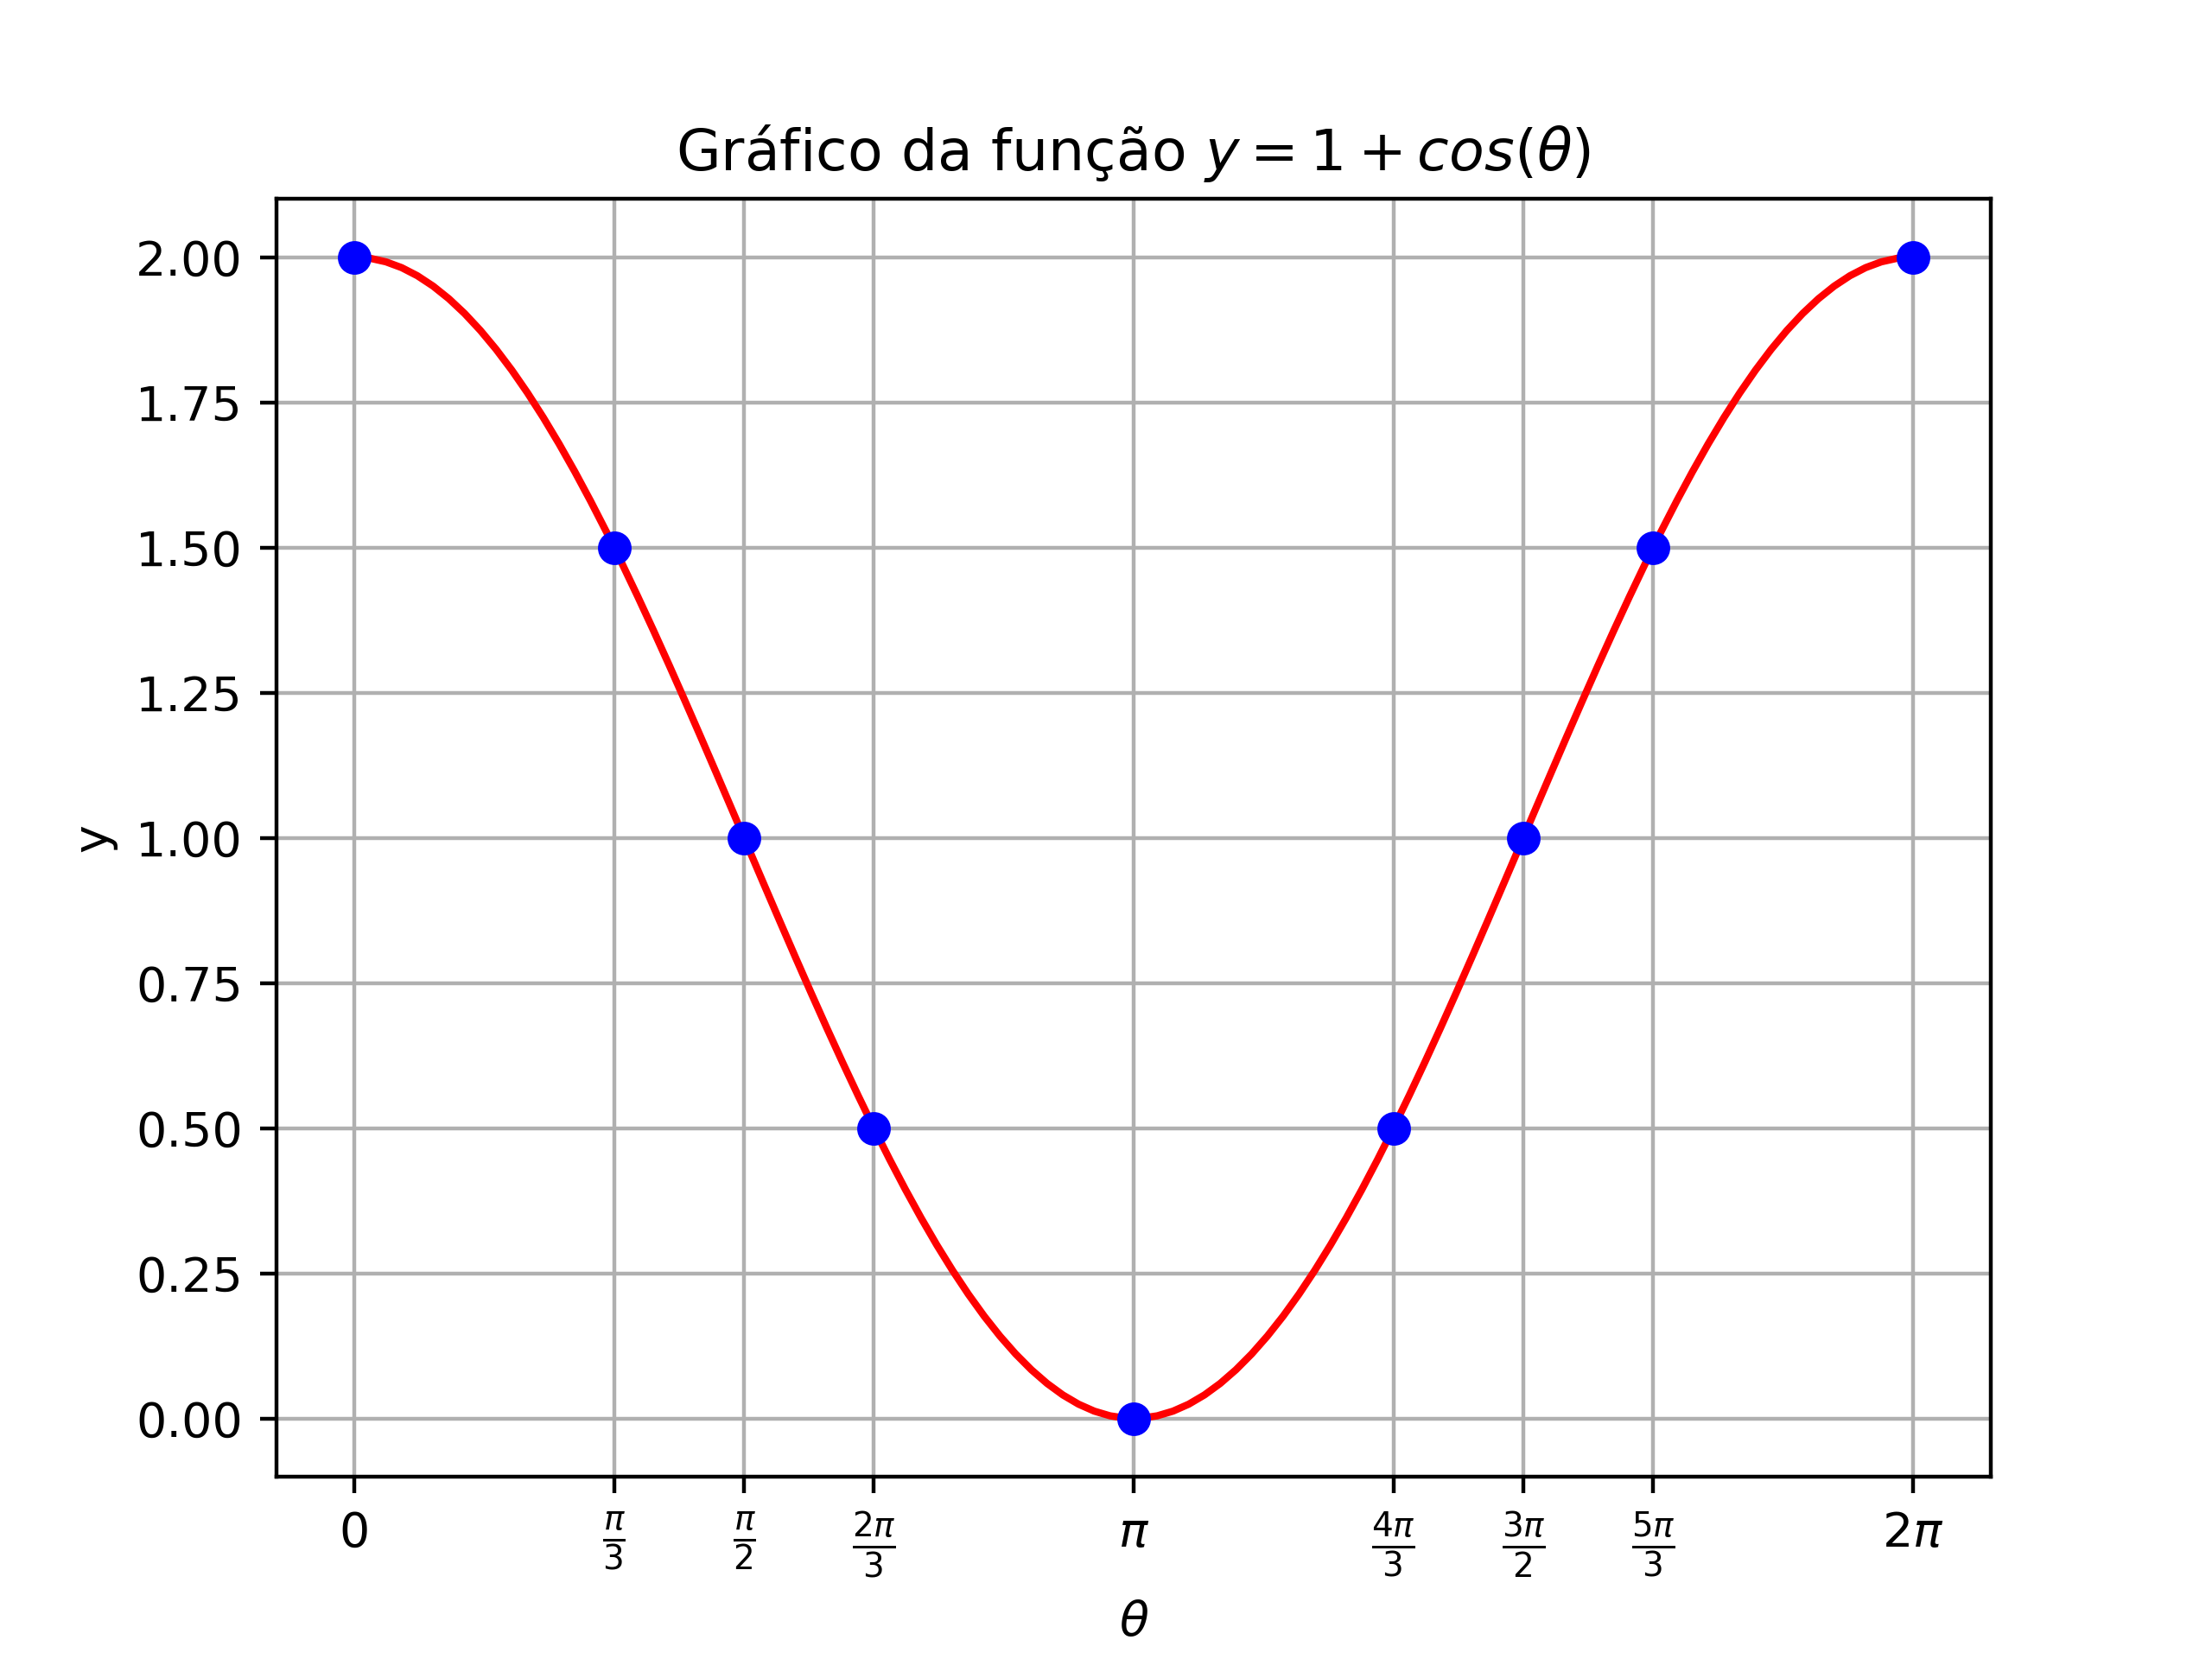
\includegraphics[scale=0.5]{figuras/grafico-aux-cardioide.png}
\end{center}
\end{frame}

\begin{frame}[label=fun-vet,fragile=singleslide]
\begin{block}{ }
\begin{pyverbatim}
import matplotlib.pyplot as plt
import numpy as np

theta= np.linspace(0, 2*np.pi, 60)
r=1+np.cos(theta)

theta=np.where(r >= 0, theta,theta + np.pi)

plt.polar(theta, np.abs(r))
plt.show()
\end{pyverbatim}
\end{block}


\end{frame}


\begin{frame}[label=fun-vet]
%\only<1>{\begin{figure}
%\centering
%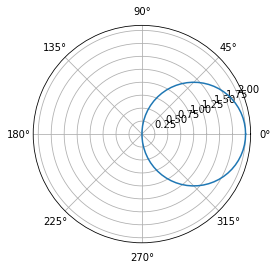
\includegraphics[scale=.7]{figuras/polar-circ.png}
%\caption{$r=2\cos \theta$}
%\end{figure}}
\only<1>{\begin{figure}
\centering
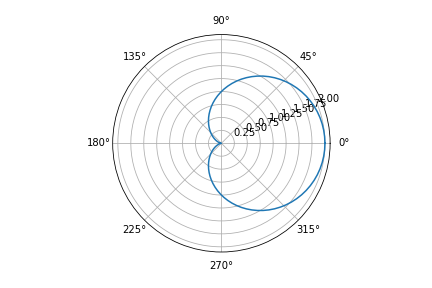
\includegraphics[scale=.7]{figuras/polar-card.png}
\caption{$r=1+\cos\theta$}
\end{figure}}
%\only<3>{\begin{figure}
%\centering
%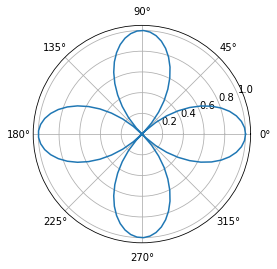
\includegraphics[scale=.7]{figuras/polar-rosasea.png}
%\caption{$r=\cos 2\theta$}
%\end{figure}}
\end{frame}

\begin{frame}[label=fun-vet]{Usando coordenadas Polares para Parametrizar}
Se em uma equação polar conseguirmos escreve a coordenada $r$ em função de $\theta$, isto é, $r=f(\theta)$, então podemos usar $\theta$ como parâmetro e parametrizar a curva representada pela equação polar da seguinte forma:
\[\vec{\alpha}(\theta)=f(\theta)(\cos \theta,\sin \theta)\]

\begin{exe}
Uma parametrização da cardioide $r=1+\cos \theta$ 
\[\vec{\alpha}(\theta)=(r\cos \theta,r\sin \theta)=(1+\cos (\theta))(\cos \theta,\sin \theta),\ \theta\in [0,2\pi].\]

\end{exe}
\end{frame}

\begin{frame}[label=fun-vet]
	\begin{casa}
		
		Esboce a curva que é representada pelas equações polares abaixo.
\begin{enumerate}
\item $r=2\cos\theta$
	
\item $r=\cos 2\theta$ (rosácea de quatro pétalas)
\end{enumerate}
	\end{casa}
\end{frame}


%\begin{frame}[label=fun-vet]
%	\begin{casa}
%		 Faça os seguintes exercícios da seção 10.3 de \cite{Stewart}
%			1, 3, 7, 9, 11, 15, 17, 19, 21, 23, 25, 29, 31, 33, 35, 37, 39, 41. 
%	
%	\end{casa}
%\end{frame}




%------------------------------------------

\begin{frame}[label=fun-vet]{Curvas Parametrizadas no espaço}
Quando uma função vetorial \dt{$\vec{r}(t)=(f(t),g(t),h(t))$}, está definida em um intervalo $I$ da reta e  é \dt{contínua}, então o conjunto {\color{red}$C$} de todos os pontos $(x,y,z)$ do plano tais que
\begin{equation}\label{parametricas2}
x=\dt{f(t)},\  y=\dt{g(t)}\ \text{ e } z=\dt{h(t)}
\end{equation}
quando $t$ varia formam uma {\color{red}curva no espaço}. As equações em  {\color{red} \eqref{parametricas2}} são ditas {\color{red} equações paramétricas de $C$}, $\dt{\vec{r}}$ é dita ser uma {\color{red}parametrização de $C$} e $t$ é chamado de  {\color{red} Parâmetro}.
\begin{exe}
Determine as curvas parametrizadas por:
\begin{enumerate} 
\item $\vec{r}(t)=(1,t,2t)$, $t\in (0,1)$.
\item $\vec{r}(t)=(\cos(t),\sin(t),t)$, $t\in [0,2\pi]$.
\end{enumerate}
\end{exe}


Veja como plotar curvas parametrizadas usando python \href{https://reginaldodr.github.io/academic/posts/curvas-parametricas/curvas-parametricas.html}{\beamergotobutton{Link}}

\end{frame}

\begin{frame}[label=fun-vet]
\begin{block}{Hélices}
A curva do exemplo anterior é uma \dt{hélice}. Existem vários tipos de hélices, as mais simples são as \dt{hélices circulares com passo constante}, cuja  parametrização e dada por 
\[\vec{r}(t)=({\color{red}a}\cos(t),{\color{red}a}\sin(t),{\color{blue}b}t),\]
onde ${\color{red}a},{\color{blue}b}$ são constantes.

As hélices aparecem em diversas aplicações, como por exemplo no formato de molas e no modelo de DNA que é formado por uma dupla hélice.
\end{block}
\begin{minipage}{0.3\textwidth}
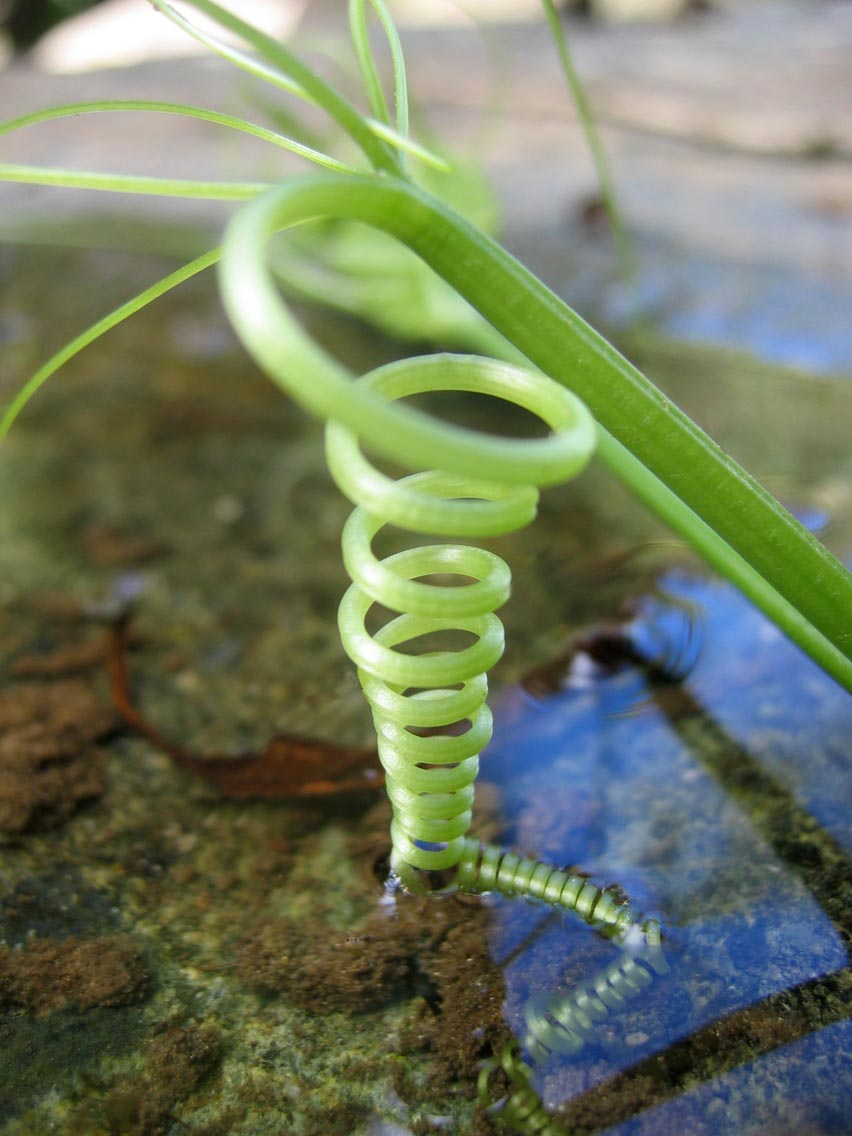
\includegraphics[scale=0.1]{figuras/DirkvdM_natural_spiral.jpg}
\end{minipage}
\begin{minipage}{0.35\textwidth}
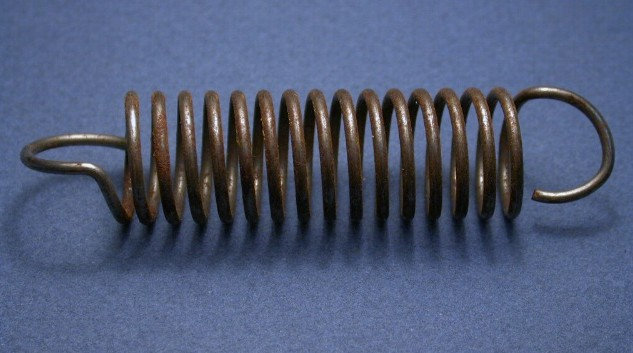
\includegraphics[scale=.7]{figuras/mola.jpg}
\end{minipage}
\begin{minipage}{0.3\textwidth}

\includegraphics[scale=.4]{figuras/dna.png}
\end{minipage}

\end{frame}



\begin{frame}[label=fun-vet]
\begin{casa}
\begin{enumerate}
\item Determine uma parametrização para o círculo de centro em $(1,2)$ e raio $3$.
\item Determine uma parametrização para o segmento de reta ligando o ponto $P=(1,3,-2)$ ao ponto $Q=(2,-1,3)$.

\item Calcule $\|\vec{r}(t)\|$, onde $\vec{r}(t)=(\cos t,\sin t, t)$, $t\in \R$.

\item Determine uma equação vetorial que represente a curva obtida pela interseção do cilindro $x^2+y^2=1$ com o plano $y+z=2$.
\item Mostre que a curva $\vec{r}(t)=(t\cos t,t\sin t,t)$ está contida no cone $z^2=x^2+y^2$ e use esse fato para esboçar a curva.
\end{enumerate}
\end{casa}
\end{frame}

\subsection*{Derivadas}
\begin{frame}[label=fun-vet]{Derivadas}
\begin{defin}
A \dt{derivada} de uma função vetorial $\vec{r}$ é definida por:
\[\frac{d\vec{r}}{dt}=\vec{r}\,'(t)=\lim\limits_{h\to 0}\frac{\vec{r}(t+h)-r(t)}{h},\]
se esse limite existir.
\end{defin}
\begin{block}{Interpretação Geométrica}
O vetor $\vec{r}\,'(t)$ é um \dt{vetor tangente} à curva parametrizada por $\vec{r}$ no ponto $P=\vec{r}(t)$.
\end{block}


\end{frame}

\begin{frame}[label=fun-vet]
\begin{prop}
Se $\vec{r}(t)=\left(f_1(t),\ldots,f_n(t)\right)$, onde $f_i$, com $i=1,\ldots,n$, são funções deriváveis, então
\[\vec{r}\,'(t)=\left(f_1'(t),\ldots,f_n'(t)\right)\]
\end{prop}

\begin{exe}
Encontre o vetor tangente unitário no ponto $t=0$ da curva 
\[\vec{r}(t)=\left(1+t^3,te^{-t},\sin(2t)\right).\]
\end{exe}
\end{frame}

\subsection*{Regras de Derivação}
\begin{frame}[label=fun-vet]{Regras de Derivação}
\begin{prop}
Sejam $\vec{u}$ e $\vec{v}$ funções vetoriais diferenciáveis, $c$ uma constante e $f$ uma função real. Então,
\begin{enumerate}
\item $\frac{d}{dt}\left(\vec{u}(t)+\vec{v}(t)\right)= \vec{u}\,'(t)+\vec{v}\,'(t)$
\item $\frac{d}{dt}\left(c\vec{u}(t)\right)= c\vec{u}\,'(t)$
\item $\frac{d}{dt}\left(f(t)\vec{u}(t)\right)= f'(t)\vec{u}(t)+f(t)\vec{u}\,'(t)$
\item $\frac{d}{dt}\left(\vec{u}(t)\cdot \vec{v}(t)\right)= \vec{u}\,'(t)\cdot\vec{v}(t)+\vec{u}(t)\cdot\vec{v}\,'(t)$
\item $\frac{d}{dt}\left(\vec{u}(t)\times \vec{v}(t)\right)= \vec{u}\,'(t)\times\vec{v}(t)+\vec{u}(t)\times\vec{v}\,'(t)$
\item $\frac{d}{dt}\left(\vec{u}(f(t))\right)= f'(t)\vec{u}\,'(f(t))$ (regra da cadeia)
\end{enumerate}
\end{prop}


\end{frame}


\begin{frame}[label=fun-vet]
\begin{exe}
Mostre que se $\|\vec{r}(t)\|=c$ para todo $t\in I$, então $\vec{r}\,'(t)$ é ortogonal a $\vec{r}(t)$ para todo $t\in I$.
\end{exe}

\begin{center}
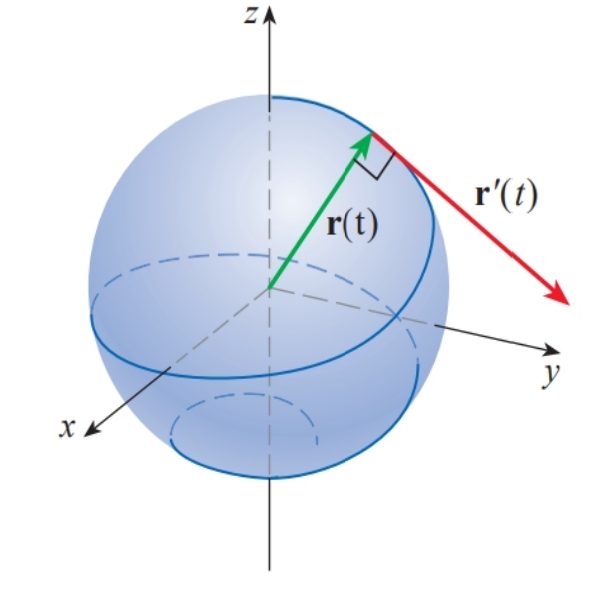
\includegraphics[scale=0.4]{figuras/vetor-const.png}
\end{center}
\end{frame}

%
%\subsection*{Integrais}
%\begin{frame}{Integral}
%A \dt{integral definida} de uma função vetorial contínua $\vec{r}$ pode ser definida da seguinte forma:
%\begin{equation*}
%	\begin{split}
%\int_a^b \vec{r}(t)\, dt & =\lim\limits_{m\to \infty}\sum_{i=1}^{m}\vec{r}(t_i^\ast)\Delta t\\
%& =\lim\limits_{m\to \infty}\left(\sum_{i=1}^{m}f_1(t_i^\ast)\Delta t,\sum_{i=1}^{n}f_2(t_i^\ast)\Delta t,\ldots,\sum_{i=1}^{n}f_n(t_i^\ast)\Delta t\right)\\
%& =\left(\int_{a}^{b}f_1(t)\,dt,\int_{a}^{b}f_2(t)\,dt,\ldots,\int_{a}^{b}f_n(t)\,dt\right)
%	\end{split}
%\end{equation*}
%\begin{exer}
%	Calcule a integral de $\vec{r}(t)=\left(2\cos(t),\sin(t)\right)$ em $[0,\pi/2]$.
%\end{exer}
%
%
%\end{frame}

\subsection*{Comprimento de arco}


\begin{frame}[label=fun-vet]{Comprimento de Arco}
	 Se {\color{red}$\vec{r}=\vec{r}(t)$}, com $a\leq t\leq b$, é curva parametrizada e {\color{red}$\vec{r}\,^\prime$ } é contínua, pode-se mostrar que o \dt{comprimento de arco} é dado por:
	\[\dt{L}=\int_a^b\|{\color{red}\vec{r}\,'(t)}\|\,dt\]
	\begin{exe}
		Um planador está voando para cima ao longo da hélice $\vec{r}(t)=(\cos(t),\sin(t),t)$. Qual a distância percorrida ao longo de sua trajetória entre os pontos $(1,0,0)$ e $(1,0,2\pi)$.
	\end{exe}
 \end{frame}


\begin{frame}
Uma mesma curva $C$ pode ser representada por mais de uma parametrização. Por exemplo, 
\[\vec{\alpha}(t)=(\cos(t),\sin(t)),\ 0\leq t\leq 2\pi\]
e
\[\vec{\beta}(t)=(\cos(2t),\sin(2t)),\ 0\leq t\leq \pi\]
ambas representam o círculo unitário com centro na origem. 

\begin{exer}
Calcule o comprimento de arco de $\vec{\alpha}=\vec{\alpha}(t)$ e $\vec{\beta}=\vec{\beta}(t)$.
\end{exer}
\end{frame}


\subsection*{Parametrização Pelo Comprimento de Arco}
\begin{frame}[label=fun-vet]{Função Comprimento de Arco}
Seja $C$ uma curva parametrizada por $\vec{r}=\vec{r}(t)$, $a\leq t\leq b$, onde $\vec{r}\,^\prime$ é contínua. Definimos a sua {\color{blue} função comprimento de arco} por
\[s(t)=\int_a^t\|\vec{r}\,^\prime (u)\|du.\]

Note que 
\[\frac{ds}{dt}=\|\vec{r}\,^\prime (t)\|\geq 0,\]
assim $s=s(t)$ é uma {\color{red}função crescente} e de classe $C^1$. Neste caso, $s$ possui uma inversa, denotada por $t=t(s)$.

\end{frame}


\begin{frame}[label=fun-vet]{Parametrização pelo Comprimento de Arco}
Isso nos permite {\color{red} reparametrizar a curva $C$ em relação ao comprimento de arco} fazendo
\[\vec{r}(s)=\vec{r}(t(s)),\ 0\leq s\leq L,\]
onde $L$ é o comprimento final da curva.

\begin{block}{ }
É frequentemente útil usar a parametrização em relação ao comprimento de arco, pois este não depende do sistema de coordenadas nem da parametrização.
\end{block}
\end{frame}

\begin{frame}[label=fun-vet]
\begin{exe}
Reparametrize a hélice circular $\vec{r}(t)=(\cos(t),\sin(t),t)$ utilizando o comprimento de arco a partir do ponto $(1,0,0)$.
\end{exe}


\begin{block}{}
Quando a curva está parametrizada pelo comprimento de arco, geometricamente isso significa que o ponto $\vec{r}(s)$  é o ponto da curva que está a $s$ unidades de comprimento do início da curva.
\end{block}
\end{frame}

\begin{frame}[label=fun-vet]
\begin{casa}
Seja $\vec{r}(t)=(e^t\sin(t),e^t\cos(t),\sqrt{2}e^t)$ e $P=(0,1,\sqrt{2})$. 
\begin{enumerate}
\item Encontre a função comprimento de arco da curva medida a partir do ponto $P$ na direção crescente de $t$.
\item Reparametrize a curva com relação ao comprimento de arco começando de $P$.
\item Encontre o ponto a 4 unidades de $P$ ao longo da curva na direção crescente de $t$.
\end{enumerate}
\end{casa}
\end{frame}

\subsection*{Curvatura}
\begin{frame}[label=fun-vet]{Vetor Tangente Unitário}
Uma parametrização {\color{red} $\vec{r}=\vec{r}(t)$} é chamada {\color{blue} suave} em um intervalo $I$ se {\color{red}$\vec{r}\,^\prime$} for contínua e {\color{red}$\vec{r}\,^\prime(t)\neq \vec{0}$} em $I$.
\medskip

Se $C$ é uma curva parametrizada por $\vec{r}=\vec{r}(t)$ suave, então o {\color{blue}vetor tangente unitário} é definido por:
\[\vec{T}(t)=\frac{\vec{r}\,^\prime(t)}{\|\vec{r}\,^\prime(t)\|}.\]


\begin{minipage}{0.5\textwidth}
O vetor tangente unitário indica a direção da curva e muda de direção muito devagar quando a curva $C$ é razoavelmente reta, mas muda mais rapidamente quando se dobra mais acentuadamente.
\end{minipage}
\begin{minipage}{0.4\textwidth}
\begin{center}
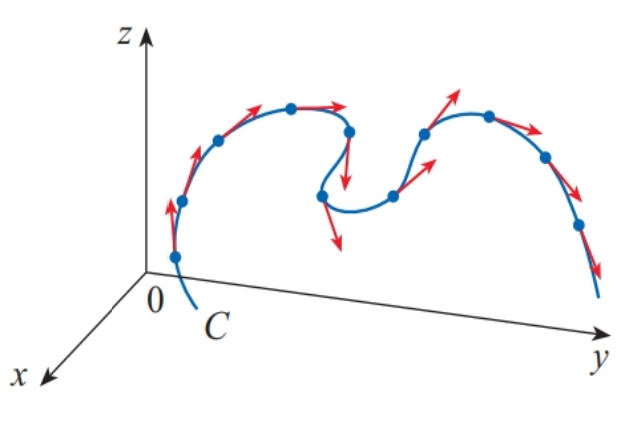
\includegraphics[scale=0.35]{figuras/vetor-tangente.png}
\end{center}
\end{minipage}

\end{frame}


\begin{frame}[label=fun-vet]{Curvatura}
A {\color{blue}curvatura} de $C$ em dado ponto é definida como 

\begin{center}
{\color{red}a taxa de variação da direção do vetor tangente unitário por unidade de comprimento,}
\end{center}
em outras palavras,
\begin{center}
{\color{red} a medida de quão rapidamente a curva muda de direção no ponto}.
\end{center} 

Por isso, definimos a curvatura como a norma  da taxa de variação do vetor tangente unitário com relação ao comprimento de arco, a saber, 
\[
\kappa(s)=\left\|\frac{d\vec{T}(s)}{ds}\right\|,
\]
onde $\vec{T}$ é o vetor tangente unitário.
\end{frame}

\begin{frame}[label=fun-vet]
Entretanto, na maioria das vezes a curva não está parametrizada pelo comprimento de arco. Neste caso, podemos usar a Regra da Cadeia para obter uma fórmula em termos de um parâmetro qualquer. Se $s=s(t)$ é a função comprimento de arco, então:
\[\frac{d\vec{T}(s(t))}{dt}=\frac{d\vec{T}(s)}{ds}\frac{ds}{dt}=\frac{d\vec{T}}{ds}\|\vec{r}\,^\prime(t)\|.\]
Logo,
\[{\color{red} \kappa(t) =\frac{\|\vec{T}\,^\prime(t)\|}{\|\vec{r}\,^\prime(t)\|}.}\]

\begin{exe}
Calcule a curvatura de um círculo de raio $\rho$.
\end{exe}
\end{frame}


\subsection*{Vetores Normal Principal e Binormal}
\begin{frame}[label=fun-vet]{Vetor Normal Principal e Binormal}
\begin{minipage}{0.7\textwidth}
Como $\vec{T}$ é unitário, sabemos que $\vec{T}$ é ortogonal à  $\vec{T}\,^\prime$, portanto definimos o {\color{blue} vetor normal unitário principal} ou simplesmente  {\color{blue} vetor normal unitário} como 
\[\color{red} \vec{N}(t)=\frac{\vec{T}\,^\prime(t)}{\|\vec{T}\,^\prime(t)\|}.\]
Veremos que este vetor indica a direção que na qual a curva está virando em cada ponto. A partir dele, definimo o {\color{blue} vetor binormal unitário}
\[\color{red} \vec{B}(t)=\vec{T}(t)\times \vec{N}(t).\]
\end{minipage}
\begin{minipage}{0.25\textwidth}
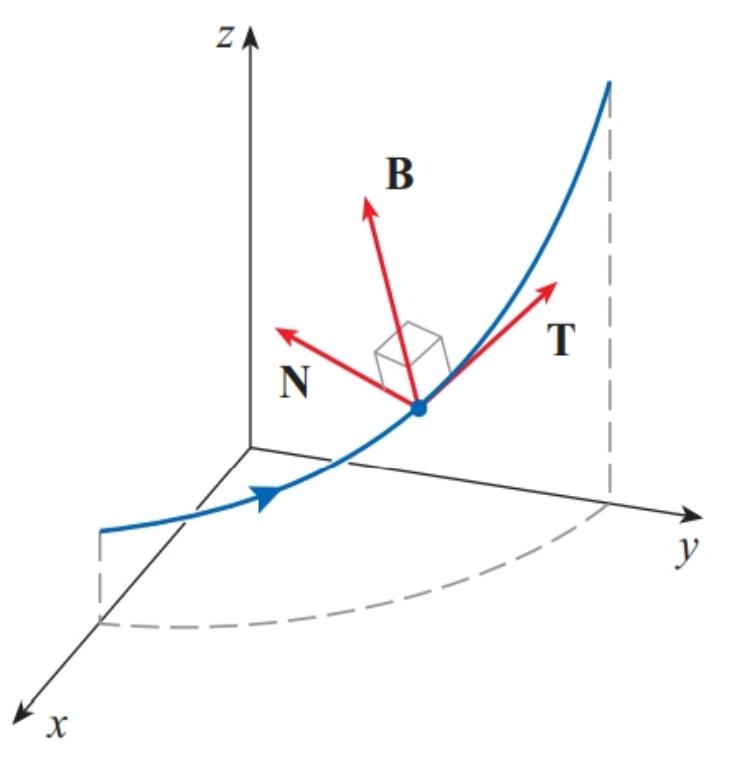
\includegraphics[scale=0.2]{figuras/normal-binormal.png}
\end{minipage}
Estes três vetores formam uma base ortonormal muito importante em geometria diferencial e no estudo de movimento de corpos, chamada de {\color{blue} Triedro de Frenet}.

\end{frame}

\begin{frame}[label=fun-vet]
\begin{exe}
Determine os vetores normal e binormal da hélice circular $$\vec{r}(t)=(\cos(t),\sin(t),t).$$

\end{exe}
\end{frame}

%\begin{frame}[label=fun-vet]
%\begin{casa}
%\begin{enumerate}
%\item Calcule a curvatura de uma reta.
%\item Calcule a curvatura de uma elipse $\frac{x^2}{a^2}+\frac{y^2}{b^2}=1$.
%\end{enumerate}
%\end{casa}
%
%
%\end{frame}

\subsection*{Movimento de partículas}
\begin{frame}[label=fun-vet]{Movimento: velocidade e aceleração}
	Suponha que uma partícula se mova de forma que seu vetor posição no instante $t$ seja $\vec{r}(t)$. Então vamos denotar por:
	\begin{itemize}
		\item $\vec{v}(t)=\vec{r}\,'(t)$ é o vetor \dt{velocidade da partícula} no instante $t$.
		\item $v(t)=\|\vec{v}(t)\|$ é a \dt{velocidade escalar} da partícula no instante $t$.
		\item $\vec{a}(t)=\vec{r}\,''(t)$ é o vetor \dt{aceleração} da partícula no instante $t$.
		\item $a(t)=\|\vec{a}(t)\|$ a aceleração escalar da partícula no instante $t$.
	\end{itemize}

\end{frame}


\begin{frame}[label=fun-vet]
Podemos mostrar que  a aceleração é dada por:
\[{\color{red}\vec{a}=v'\vec{T}+v^2\kappa \vec{N}. }\]
Com isso temos as seguintes conclusões:
\begin{itemize}
\item O vetor $\vec{B}$ não aparece, ou seja, a aceleração sempre está no plano determinado por $\vec{T}$ e $\vec{N}$, chamado {\color{blue} plano osculador}.


\item A componente tangencial da aceleração mede a taxa de variação do módulo da  velocidade, isto é, a mudança na velocidade escalar.

\item A componente normal é dada pelo quadrado da velocidade escalar e pela curvatura.
\end{itemize}

\begin{exe}
Um objeto de massa $m$ que se move em uma trajetória circular com velocidade angular constante $\omega$ tem vetor posição dado por $\vec{r}(t)=(\rho\cos (\omega t), \rho\sin (\omega t)).$ Determine a força que age sobre o objeto.
\end{exe}
\end{frame}


\subsection*{Fórmula para a curvatura}
\begin{frame}[label=fun-vet]
Usando a última equação, podemos deduzir a seguinte fórmula para a curvatura.
\begin{teo}
A curvatura de uma curva parametrizada suave $\vec{r}=\vec{r}(t)$ é dada por:
\[\kappa(t)=\frac{\|\vec{v}(t)\times \vec{a}(t)\|}{v^3(t)}=\frac{\|\vec{r}\,^\prime(t)\times \vec{r}\,^{\prime\prime}(t)\|}{\|\vec{r}\,^\prime(t)\|^3}.\]
\end{teo}

\begin{exe}
Determine a curvatura da cúbica retorcida $\vec{r}(t)=(t,t^2,t^3)$.
\end{exe}
\end{frame}


\begin{frame}[label=fun-vet]
	\begin{casa}
		\begin{enumerate}
		
	\item  Mostre que a curvatura de uma curva plana que tem equação cartesiana da forma $y=f(x)$ é dada por:
	\[\kappa(x)=\frac{|f''(x)|}{\left(1+[f'(x)]^2\right)^{3/2}}.\]
		
	\item Calcule a curvatura da parábola $y=x^2$ e determine o ponto onde a curvatura é máxima.
	
	\item Determine as componentes normal e tangencial da aceleração da partícula que se move segundo a trajetória $\vec{r}(t)=e^{-t}\,\vec{i}+e^t\,\vec{j}$.
	
	\item Uma partícula se move sobre a parábola $y=x^2$ da esquerda para a direita. Quando ela passa pelo ponto $(2,4)$, sua velocidade é $v=3$ m/s e $v'=7$ m/s$^2$. Ache o vetor velocidade e o vetor aceleração neste ponto.
	
	
%	\item Determine as componentes tangencial e normal do vetor aceleração da curava 
	%\[\vec{r}(t)=(t^2+1)\vec{i}+t^3\vec{j}, \ t\geq 0.\]
		

%\item Determine uma parametrização para a reta tangente à hélice $\vec{r}(t)=\left(2\cos t,\sin t, t\right)$ no ponto $P=(0,1,\pi/2)$.
%			
%			\item Determine o comprimento de arco da cardioide $r=2(1+\cos \theta)$.
%			
%			\item Determine os vetores velocidade e aceleração e a velocidade escalar da partícula cuja função posição é 
%			\[\vec{r}(t)=3\cos(t)\,\vec{i}+2\sin( t)\, \vec{j},  0\leq t\leq 2\pi.\]
%			Faça um esboço da trajetória e marque os vetores velocidade onde a velocidade escalar é mínima e máxima.
		\end{enumerate}
	\end{casa}
\end{frame}




